\documentclass[12pt]{article}
\addtolength{\oddsidemargin}{-.875in}
	\addtolength{\evensidemargin}{-.875in}
	\addtolength{\textwidth}{1.75in}

	\addtolength{\topmargin}{-.875in}
	\addtolength{\textheight}{1.75in}
\usepackage{epsfig}
\usepackage{graphicx}
\usepackage{amsthm, amsmath}
\usepackage{amsfonts}
\usepackage{color}
\usepackage{enumitem}

%\numberwithin{equation}{section}

\newcommand{\field}[1]{\mathbb{#1}}
\newcommand{\R}{\field{R}}
\newcommand{\F}{\field{F}}
\newcommand{\p}{\field{P}}
\newcommand{\N}{\field{N}}
\newcommand{\Z}{\field{Z}}
\newcommand{\X}{\field{X}}
\newcommand{\E}{\field{E}}
\newcommand{\W}{\field{W}}
\newcommand{\B}{\field{B}}

\def\qed{\hfill$\diamondsuit$}
\def\II{I\negthinspace I}
\def\B{I\negthinspace\negthinspace B}
\def\ccirc{\negthinspace\circ}
\def\median{\mathop{\mbox{med}}}
\def\argmax{\mathop{\mbox{argmax}}}
\def\argmin{\mathop{\mbox{argmin}}}
\theoremstyle{Conjecture}
\theoremstyle{example}
\theoremstyle{remark}
\theoremstyle{lemma}
\theoremstyle{definition}
\theoremstyle{corol}
\theoremstyle{proposition}
\theoremstyle{condition}
\newtheorem{theorem}{Theorem}
\newtheorem{example}{Example}
\newtheorem{remark}{Remark}
\newtheorem{lemma}{Lemma}
\newtheorem{definition}{Definition}
\newtheorem{corol}{Corollary}
\newtheorem{condition}{Condition}
\newtheorem{proposition}{Proposition}
\newtheorem{Conjecture}{Conjecture}


\def\cod{\stackrel{\cal D}{\longrightarrow}}
\def\cop{\stackrel{\cal P}{\longrightarrow}}
\def\eqd{\stackrel{\cal D}{=}}
\def\eqp{\stackrel{\cal P}{=}}
\def\ap#1{\smash{\mathop{\approx}\limits^{#1}}}
\def\lf{\lfloor}
\def\rf{\rfloor}
\def\lc{\lceil}
\def\rc{\rceil}
%\def\N{{\open N}}
%\def\Z{{\open Z}}

\oddsidemargin -0pt
\evensidemargin -0pt
\topmargin -20pt
\textheight 630pt
\textwidth 460pt
\renewcommand{\baselinestretch}{1.3}
\begin{document}

\bibliographystyle{plain}

\begin{center}
Midterm Exam: STAT 380, Spring 2017\\ Penn State
\end{center}
\begin{flushleft}
NAME
\end{flushleft}
I have neither given nor received any assistance in the taking of this exam. \\
Signature: \\\\
Instructions: 
\begin{enumerate}
\item This is a closed book exam. 
%You are only allowed one 8.5 inch$\times$11 inch sheet of notes and a calculator.
%\item Please show all your work and write clearly for full credit.
%\item `Box' your final answer to each question (draw a box around it).
% \item You may leave your answer unsimplified,e.g. $0.7^{4}
% \frac{18!}{4!8!}, 14 e^{-23}, 1.67-0.938$.
\item {\it Turn off all electronic devices}!  Any student whose 
electronic device rings, vibrates, or makes any sound during 
the exam shall turn in their paper and leave the room immediately.
\item Please verify that your exam paper contains all 6 questions.
% \item You may use a calculator and one sheet of notes.  You may
% {\it not} use any books or share a calculator with another student.
%\item Illegible handwriting will not be graded!
\item To earn credit, write clearly, and show your work. When in
  doubt, explain things clearly. If you need extra paper then please write on
  the back of your paper.
% \item {\it The instructors or teaching assistants will answer no
% questions during the exam period.}  Simply explain any error
% you may find in a question and proceed to the next question.
\end{enumerate}
\centerline{DO NOT WRITE BELOW THIS LINE}

\vskip 0.1truein

\centerline{\vbox{\offinterlineskip
\halign{&\vrule#&\hfil\ #\hfil\cr
\noalign{\hrule} \cr
height10pt&\omit && \omit &\cr
& Question && Marks &\cr
height10pt&\omit && \omit &\cr
\noalign{\hrule} \cr
height10pt&\omit && \omit &\cr
& 1 && {\hskip40pt} &\cr
height10pt&\omit && \omit &\cr
\noalign{\hrule} \cr
height10pt&\omit && \omit &\cr
& 2 && {\hskip40pt} &\cr
height10pt&\omit && \omit &\cr
\noalign{\hrule} \cr
height10pt&\omit && \omit &\cr
& 3 && {\hskip40pt} &\cr
height10pt&\omit && \omit &\cr
\noalign{\hrule} \cr
height10pt&\omit && \omit &\cr
& 4 && {\hskip40pt} &\cr
height10pt&\omit && \omit &\cr
\noalign{\hrule} \cr
height10pt&\omit && \omit &\cr
& 5 && {\hskip40pt} &\cr
height10pt&\omit && \omit &\cr
\noalign{\hrule} \cr
height10pt&\omit && \omit &\cr
& 6 && {\hskip40pt} &\cr
height10pt&\omit && \omit &\cr
\noalign{\hrule} \cr
height10pt&\omit && \omit &\cr
% & 7 && {\hskip40pt} & \cr
% height10pt&\omit && \omit &\cr
% \noalign{\hrule} \cr
% \noalign{\hrule} \cr
% height10pt&\omit && \omit &\cr
& Total && {\hskip40pt} & \cr
height10pt&\omit && \omit &\cr
\noalign{\hrule} \cr}}}

\newpage 

\begin{enumerate}

%%
 \item[Q1] 
%\resizebox{10ex}{2\baselineskip}{Dunhill style}
%\scalebox{10}{Giant}
%\framebox[3\width]{Guess I’m framed now!}
(16 pts) The Behavioral Risk Factor Surveillance Survey: is conducted
biannually. We have the data from 1970 and 1990. The following
measurements were made on each individual surveyed:
\begin{itemize}
\item weight: measured in pounds, with a value of 999 for missing
\item height: measured in inches
\item age: measured in years
\item daysSick: number of days in the past 30 days that health was not good. Values include 1 to 30. None is coded as 88.
\item lastCheckup: time since last routine checkup. Values are 1 for within a year, 2 for more than 1 and less than 2 years, 3 for more than 2 and less than 5 years, 4 for more than 5 years, and NA for don’t know.
\item phone: the respondent was contacted by land line (1) or cell
  phone (2).
\end{itemize}

The data are in a data frame called BRFSS. To prepare the data for
analysis, write code to perform each of the following operations. 
\begin{enumerate}%[label=\alph*]
\item Recode the number of days sick so that 88 is 0.
\begin{verbatim}
	BRFSS$daysSick[BRFSS$daysSick == 88] <- 0
\end{verbatim}
\vspace{0.4in}
\item Convert a weight of 999 to NA.
\begin{verbatim}
	BRFSS$weight[BRFSS$weight == 999] <- NA
\end{verbatim}
\vspace{0.4in}
\item Turn lastCheckup into a factor with appropriate labels for the levels.
\begin{verbatim}
	BRFSS$lastCheckup <- factor(BRFSS$lastCheckup,
								labels = c(`less than 1 yr', `1-2 yrs', `2-5 yrs', `more than 5 yrs'))
\end{verbatim}
\vspace{0.4in}
\item Drop all records from the data frame that have a value of NA for the time of the last check up. (Assign the smaller data frame to BRFSS2).
\begin{verbatim}
	BRFSS2 <- BRFSS[!is.na(BRFSS$lastCheckup), ]
\end{verbatim}
\end{enumerate}

\newpage

\item[Q2] (20 pts) Write a function called qcd(), short for quartile
  coefficient of dispersion. This function takes two arguments: the
  required $x$, which is a numeric vector; and the optional na.rm,
  which indicates whether NAs should be removed from $x$. The default
  value for this argument should be FALSE. The function returns the
  single numeric value that is the ratio of the interquartile range
  (=75th percentile-25th percentile) to the sum of the lower (25th
  percentile) and upper (75th) percentiles. Note: the function IQR(x,
  na.rm=FALSE) returns the interquartile range of the vector x. Also,
  the function quantile(x, 0.25) returns the 25th percentile. In
  addition, check that the input for x is numeric and if not terminate
  execution and provide an informative error message.

  \begin{verbatim}
qcd <- function(x, na.rm = FALSE) {
    if(!is.numeric(x)) stop(`x must be a number')
    if(na.rm) x <- x[!is.na(x)]
    iqr <- IQR(x, na.rm = na.rm)
    q25 <- quantile(x, 0.25)
    q75 <- quantile(x, 0.75)
    return(iqr/(q25 + q75))
}
  \end{verbatim}

\newpage
\item[Q3] (16 pts) What is the value printed to the console for each
  of the following expressions?
\begin{enumerate}
\item 
% \begin{verbatim} 
\begin{verbatim}
 > x = c(-1, -1, -1, -1, 1, -1) 
 > y = cumsum(x) 
 > y 
\end{verbatim}
\vspace{.5in}
\begin{verbatim}
[1] -1 -2 -3 -4 -3 -4
\end{verbatim}
\vspace{.5in}
\item 
\begin{verbatim}
 > z = which(y < -10) 
 > z
\end{verbatim}
\vspace{.5in}
\begin{verbatim}
integer(0)
\end{verbatim}
\vspace{.5in}
\item 
\begin{verbatim}
 > z[length(z)]
\end{verbatim}
\vspace{.5in}
\begin{verbatim}
integer(0)
\end{verbatim}
\vspace{.5in}
\item 
\begin{verbatim}
> x[z]
\end{verbatim}
\vspace{.5in}
\begin{verbatim}
numeric(0)
\end{verbatim}
\vspace{.5in}
\end{enumerate}

\newpage

% \item[Q4] (12 pts) For the following function call show the steps in the computations that R carries out.\\
%  afunc(1:4, 10:13)
\item[Q4] (12 pts) Write a function that uses Monte Carlo to
  approximate the distribution of the sample proportion of Heads from
  $n$ coin tosses of a coin (which may or may not be a fair coin). The
  function should take as input the sample size $n$, the probability
  of heads $p$, the number of replicates (repetitions of the experiment)
  $B$ and a boolean {\tt plotHist} that if TRUE prints a histogram of
  the samples and if not, does not. If the user does not input a value
  for $B$, default to the one we often use in class, that is, set
  $B=10,000$. The output of the function should be the mean and
  standard deviation of the distribution.

  \begin{verbatim}
mc <- function(n, p, B = 10000, plotHist = TRUE) {
    numHeads <- rep(NA, B)
    for(i in 1:B) {
        flips <- sample(0:1, size = n, replace = TRUE, prob = c(1-p, p))
        numHeads[i] <- sum(flips)
    }
    if(plotHist) hist(numHeads)
    return(list(mean = mean(numHeads), sd = sd(numHeads)))
}
  \end{verbatim}

  or

  \begin{verbatim}
mc <- function(n, p, B = 10000, plotHist = TRUE) {
    numHeads <- rbinom(B, n, p)
    if(plotHist) hist(numHeads)
    return(list(mean = mean(numHeads), sd = sd(numHeads)))
}
  \end{verbatim}

 \newpage

\item [Q5] (20 pts)
\begin{enumerate}
\item Suppose you want to analyze daily temperatures at 3 different
locations and that the number of days where data are available at
these locations is quite different. What kind of data structure would
you use to store all these data and why? 

\vspace{0.25in}
\textcolor{blue}{A list. Data frames require every vector to be the same length, lists do not.}
\vspace{0.25in}

\item Suppose you have a dataset of heights (in) and weights (lbs) of adults. You know there are 25,000 rows in the data. When you make a scatterplot, this is what you see:
\begin{center}
  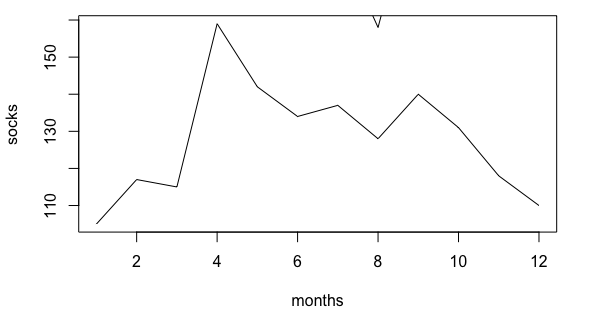
\includegraphics[width=0.8\textwidth]{plot.png}
\end{center}
\begin{enumerate}
  \item Why are there fewer than 25,000 points on the plot? What can you do to make more points visible?

  \textcolor{blue}{The data are integer valued, so many points lie on top of each other. We can ``jitter'' the points, adding a small amount of noise in all directions so that the points appear more spread out.}
  \item How can you improve this plot to make it more informative for a reader?
  \textcolor{blue}{Axis labels, specify units, plot title, ...}
\end{enumerate}
\end{enumerate}
% Consider the plot below. It exams the causes of
%  death among males at various ages. These data are from the Centers
%  for Disease Control and Prevention data base. In answering the
%  questions be sure to use the graphics terminology introduced in the
%  course.

\newpage
\item[Q6] (16pts) Consider the following list, aList:
\begin{verbatim}
aList
  $x
  [1] "a" "b" "c" "d" "e"
  $mat
       [,1] [,2]
  [1,]    8    5
  [2,]    7    4
  [3,]    6    3
$zz
$zz$x
[1] 1 2 3
$zz$y
[1] 7 8
91011
$zz$z
[1]  TRUE  TRUE FALSE FALSE  TRUE
$one [1] 100
\end{verbatim}
Write down what will appear at the console when R evaluates each of 
the following expressions (note that some expressions may result in 
an error message):
\begin{enumerate}
\item \verb| length(aList) |

\verb| [1] 4 |
\item \verb| aList$mat + aList$one|

\begin{verbatim}
     [,1] [,2]
[1,]  108  105
[2,]  107  104
[3,]  106  103
\end{verbatim}
\item \verb| length(aList[["zz"]][1])|

\verb| [1] 1 |
\item \verb| sapply(aList$zz, min)|

\begin{verbatim}
x y z 
1 7 0 
\end{verbatim}
\end{enumerate}
\end{enumerate}

\end{document}
